\documentclass{article}

\usepackage{graphicx}
\usepackage{float}
\usepackage{cite}
\usepackage{url}
\usepackage{caption}
\usepackage{subcaption}

\begin{document}

\section{Basic Camera Model}

The basic camera model is implemented inside the camera class. The camera class
allows the creation of rays for a given pixel on the image place. The class first uses the Up and
Lookat vectors to create an orthogonal basis w, u, v. A field of view is defined
and then used along with the value for the width, hight and current pixel location
to calculate the point on the camera screen that corresponds to the center of the
viewing plane.

In order to create a ray given the x and y pixel locations on the output image
the angle between the x and y axis that the ray leaves the camera position at are
calculated. These angles are easy to calculate as the field of view angle is
previously defined, this can be divided by the number of pixels to give a degree
per pixel value. This degree per pixel value can be multiplied by the pixel x, y
values to give offset angles from the camera center line. Using these angles,
the focal length and the center point of the image
plane the point the ray intersects the image plane through is found using simple
trigonometry. This image plane intersection
point can then be used to find the correct ray parameters.

In order to implement basic anti-aliasing each pixel has multiple rays fired and
averaged. In total 16 rays are fired per pixel, these rays are arranged in a regular grid across the pixel where each
ray is 0.25 pixel widths from the previous.
The colour values returned by raytracing each of these rays are then averaged to give the anti-aliased
value. Figure \ref{fig:antialias} shows a raytraced sphere with and without anti-aliasing
turned on.\\

\begin{figure}[H]
  \begin{center}
  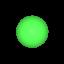
\includegraphics[width=150px]{Images/antialiasOff.png}
  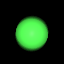
\includegraphics[width=150px]{Images/antialiasOn.png}
  \caption{Sphere raytraced with and without anti-aliasing}
  \label{fig:antialias}
  \end{center}
\end{figure}

\section{Plane \& Triangle Intersection}

The triangle intersection is done in the triangle class. The class takes three
vertexs as parameters, these are the three corners of the triangle. This first step in the
intersection test is to calculate the three vectors which make up the sides
of the triangle. Once the vectors are calculated they are used to get the normal by the application of the
cross product \cite{triangle}. Using the normal and one of the triangle vertexs
the ray intersection point can be found. This is done by firstly checking the ray
passes through the plane defined by the normal and point. If the ray does intersect
the plane the three triangle vectors can be used to check if the ray intersects
inside of the triangle bounds. In order to check the ray intersects within the
triangle three extra vectors are need, these are the ones between each vertex and
the ray intersection point. If the cross product between these vectors and the
corresponding triangle vectors are all have positive dot products then the intersection
point is within the triangle. Figure \ref{fig:triint} shows a very simple triangle
primitive.\\

\begin{figure}[H]
  \begin{center}
  
\includegraphics[width=150px]{Images/triangle.png}
  \caption{Triangle intersection}
  \label{fig:triint}
  \end{center}
\end{figure}

The plane object is in the plane class. Plane intersections is done exactly the
same way as the first half of the triangle intersection. First the normal is found
then using on of the points that define the plane the ray is checked for intersection
and a t value is found. Figure \ref{fig:plane} shows a plane and a sphere which
partially overlaps the plane.

\begin{figure}[H]
  \begin{center}
  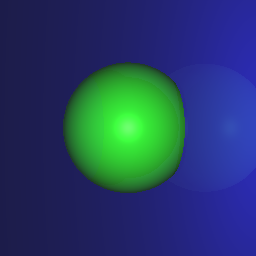
\includegraphics[width=150px]{Images/plane.png}
  \caption{Plane intersection}
  \label{fig:plane}
  \end{center}
\end{figure}


\section{Quadratic Intersection}

Quadratic surfaces are defined by 9 values and correspond to the values A - J in the equation below.
This equation enables the definition of any quadratic surface.

\begin{center}
$Ax^2 + 2Bxy + 2Cxz + 2Dx + Ey^2 + 2Fyz + 2Gy + Hz^2 + Iz + J = 0$
\end{center}

In order to calculate the intersection point between a ray and the surface the
ray equation $Dt + P = 0$ can be substituted into the quadratic. This substitution gives the
quadratic equation below where dx, dy and dz are the x,y and z components of the ray
direction and px, py and pz are the components of the initial ray position \cite{quadratic}.

\begin{center}
$Aqt^2 + Bqt + Cq = 0$ Where
$Aq = Adx^2 + Edy^2 + Hdz^2 + Bdxdy + Cdxdz + Fdydz$
$Bq = 2Apxdx + 2Epydy + 2Hpzdz + B(pxdy + pydx) + C(pxdz + pzdx) + F(pydz + pzdy) + Ddx + Gdy + Idz$
$Cq = Apx^2 + Epy^2 + Hpz^2 + Bpxpy + Cpxpz + Fpypz + Dpx + Gpy + Ipz + J$
\end{center}

This can then be solved using the quadratic equation, if there are no solutions
then the ray does not intersect the quadratic surface. Figure \ref{fig:quadsurface}
shows three quadratic surfaces, first a cylinder finded with the equation $x^2 + z^2 - 1$
, secondly a paraboid defined as $x^2 + z^2 - y$ and finally a sphere defined as
$x^2 + y^2 + z^2 - 1$.

\begin{figure}[H]
\centering
\begin{subfigure}{.3\textwidth}
  \centering
  
\includegraphics[width=100px]{Images/quadCylinder.png}
  \caption{Cylinder}
\end{subfigure}%
\begin{subfigure}{.3\textwidth}
  \centering
  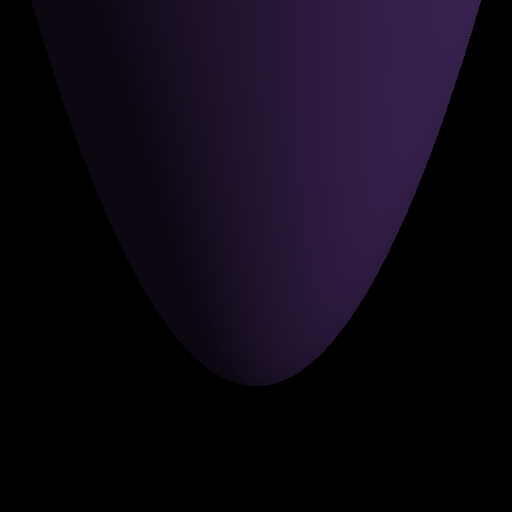
\includegraphics[width=100px]{Images/quadParaboid.png}
  \caption{Paraboid}
\end{subfigure}
\begin{subfigure}{.3\textwidth}
  \centering
  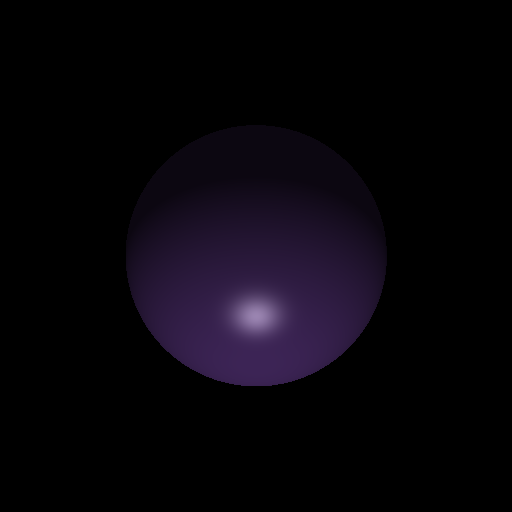
\includegraphics[width=100px]{Images/quadSphere.png}
  \caption{Sphere}
\end{subfigure}
\caption{Quadratic Surfaces}
\label{fig:quadsurface}
\end{figure}

\section{Point Lights}

Point lights are implemented in the point\_light.cpp class. The class takes a vertex
and colour as arguments as well as an optional vector for the direction of the light.
When the lights is checked with an object and intersection point if there is no direction
given the intensity of the colour returned is equal to that defined in the arguments.
When a direction has been specified the angle between the light direction and the
vector from the light to the intersection point is calculated, using the dot product.
If the dot product is negative then the intensity is 0 as the angle is more than
90 degrees. Otherwise the intensity is scaled by the value of the dot product
to the power of 0.5, which is a value to control the rate of fall off.\\

Figure \ref{fig:pointligh} shows two point lights, one red and one green,
pointed at a sphere. Not as there is a direction defined in the point light
construction the colour across the sphere is not constant.\\

\begin{figure}[H]
  \begin{center}
  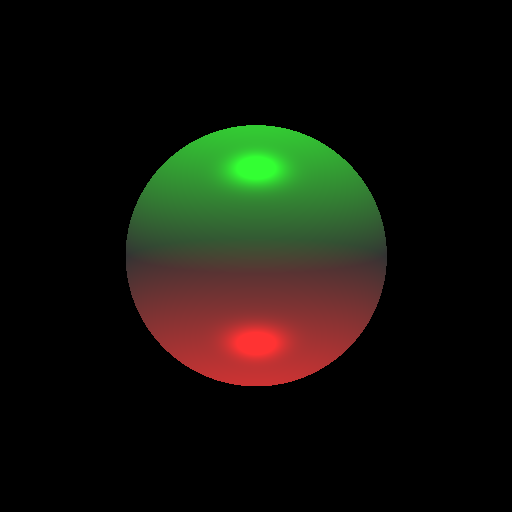
\includegraphics[width=150px]{Images/pointLight.png}
  \caption{Basic Camera Model}
  \label{fig:pointligh}
  \end{center}
\end{figure}

\section{Specular Material}

In order to show specular materials part of the intensity at a given location is
a function of the angle between the light direction and the viewing ray direction,
as defined by the Phong model. First the lights reflection ray is calculated using the
normal at the point of intersection and the vector pointing at the light source. Then
the dot product between the reflection vector and the viewing ray is used to scale the
specular component of the intensity given by the light.\\

The reflection ray of the viewing ray is also computed in order to calculate any
reflections in the surface, this is done using the viewing ray and normal.
The reflection ray is ray traced in the same way as the
primary rays and the returned colour is added to the overall intensity multiplied
by the materials reflection scaling value. A recursion depth is defined in the
camera class before raytracing starts, this thus limits the number of reflections.
Figure \ref{fig:reflectionrays} shows a set of spheres in both images the specular
component can be seen, also in the first reflections are enabled. Figure \ref{fig:reflections}
shows a more complex scene with reflections.

\begin{figure}[H]
\centering
\begin{subfigure}{.5\textwidth}
  \centering
  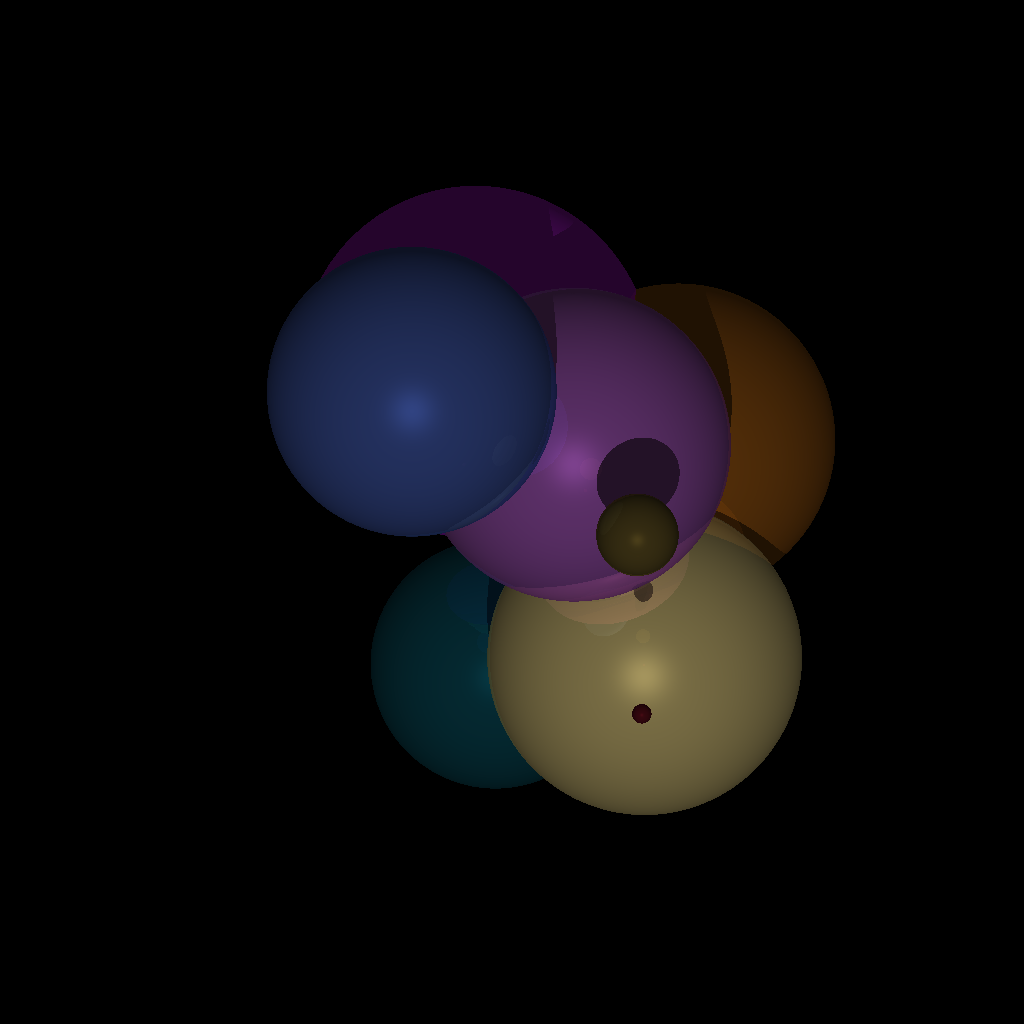
\includegraphics[width=150px]{Images/reflectionsOn.png}
  \caption{With reflection}
\end{subfigure}%
\begin{subfigure}{.5\textwidth}
  \centering
  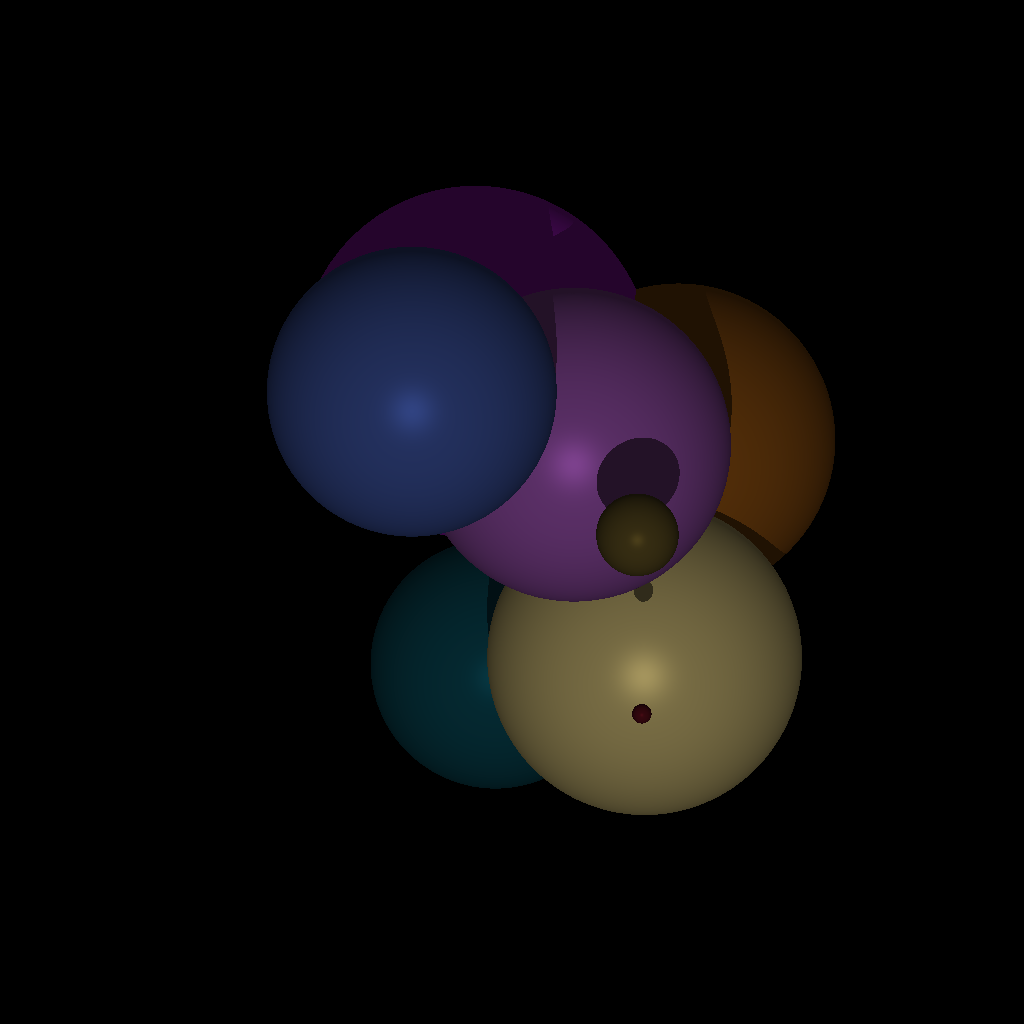
\includegraphics[width=150px]{Images/reflectionsOff.png}
  \caption{Without reflection}
\end{subfigure}
\caption{Raytraced image with and without reflection rays}
\label{fig:reflectionrays}
\end{figure}


\begin{figure}[H]
  \begin{center}
  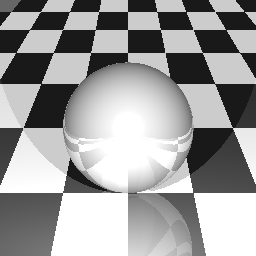
\includegraphics[width=150px]{Images/gridSphere.png}
  \caption{More reflections}
  \label{fig:reflections}
  \end{center}
\end{figure}

\section{Shadows}

Shadow rays are also computed at each intersection point with each of the lights.
At an intersection point the ray between the point and each of the lights is computed.
This ray is raytraced in a similar way to the primary rays, however we only care about whether
there is an intersection with an object. If there is an intersection it is checked
that this happens before the ray reaches the light. If there is an intersection before
the light then this point on the object is in shadow, therefore the component of the
intensity of that light is ignored. Figure \ref{fig:shadow} shows a set of spheres
shadowing each other.

\begin{figure}[H]
  \begin{center}
  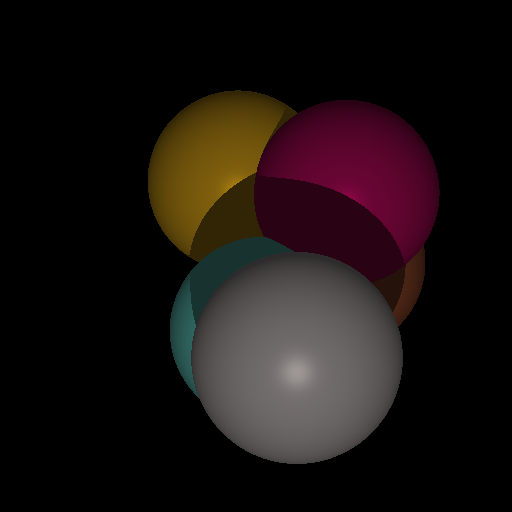
\includegraphics[width=150px]{Images/shadows.png}
  \caption{Shadow Image}
  \label{fig:shadow}
  \end{center}
\end{figure}

\section{Transparent Material}

In order to raytrace transparent materials the refracted ray must be computed at
each intersection and raytraced. The refracted ray is computed using Snells law
and then raytraced the same way as primary rays are. In order to compute the refraction
ray each object is defined a ratio of speed of light in vacuum to the speed in that
material. As the refraction ratio changes depending on whether the ray is exiting
or entering an object this needs to be computed and can be done by comparing
the dot product between the normal and the viewing ray.\\

Once the refracted ray has been raytraced the refracted component can be added
to the pixel value, multiplied by a scaling value. Some transparent surfaces
can have more complex relationships between the transparent and reflective
scaling values. This means as the angle between the normal and the viewing ray increases
the transparent component decreases and the reflective increases. In order to
compute this the Fresnel equation is used to scale the kr and kt values accordingly.
Figure \ref{fig:trans} shows a transparent sphere on top of a grid of squares.
The grid can be seen distorted by the sphere.
\begin{figure}[H]
  \begin{center}
  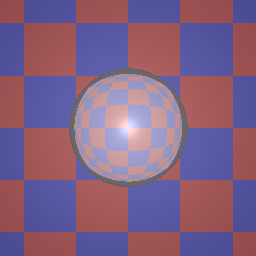
\includegraphics[width=150px]{Images/transparent.png}
  \caption{Transparent Sphere}
  \label{fig:trans}
  \end{center}
\end{figure}
\newpage
\section{Octree}

In order to improve the performance of the raytracer an octree was implemented.
This consists of breaking the scene down into a set of axis aligned bounding
boxes. The boxes make up a tree with each node having eight child
boxes, one root box is defined and covers the whole scene.
The tree building algorithm is recursive firstly starting by splitting
the root box, then its children and so on until the limit of tree depth is
reached. Each time a box is added to the tree all the objects in the scene area
checked for there intersection with the box. If a box does not contain any objects
it becomes a leaf node. Once the depth limit is reached then all leaf nodes have a list
of objects which are inside compiled. Each object has a intersect with bounding
box method, this is used to check if the object exists inside the bounding box or
not. Currently only triangles and spheres have this method all others simply return
true. This was due to time restrictions and the fact triangles and spheres are
enough to show the octree algorithm works successfully.\\

When raytracing a ray, intersections the octree is searched for node boxes that the ray passes through.
This is done starting with the root node and then its children. If at any point a
box does not intersect then none of its children need checking. When a
leaf node is found that the ray passes through, all the objects in that box
are tested for intersections. To avoid objects which overlap bounding boxes
being tested twice each object has a property which records the last ray number
that it was tested with, if this is equal to the current ray the object is
skipped. Ray numbers are simply the result returned from the clock() function
when the ray was created, as the clock function returns the clock ticks since
program start this gives a unique value for each ray.\\

This improves performance significantly, the image in figure \ref{fig:octree}
is a 256 x 256 image and takes 53 seconds to compute without an octree.
With an octree enables this time is reduced to 9 second.

\begin{figure}[H]
  \begin{center}
  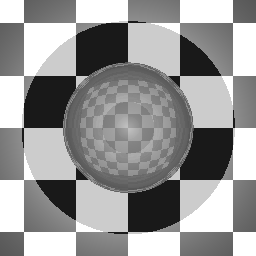
\includegraphics[width=150px]{Images/octreeTest.png}
  \caption{Basic Camera Model}
  \label{fig:octree}
  \end{center}
\end{figure}

\bibliographystyle{unsrt}
\bibliography{ref}

\end{document}